\chapter{Resultados}\label{cap:4}
\lettrine{E}{ste apartado presenta las simulaciones} realizadas a lo largo del desarrollo del proyecto, así como las principales observaciones y análisis de las imágenes obtenidas. Además, también aparecen fragmentos de los códigos y programas que participan, incluyendo los parámetros introducidos o modificados protagonistas de las diferentes secciones que componen este cuarto capítulo \S\ref{cap:4} dedicado a los resultados.

En primer lugar, antes de iniciar el proceso de análisis, es necesario hacer una pequeña introducción orientada a introducir los parámetros ---tanto los fijos como los variables--- y contextualizar las motivaciones que llevaron a realizar los cambios en los perfiles de densidad de \ce{Kr^{8+}} y densidad electrónica. El objetivo es reproducir adecuadamente los perfiles radiales de intensidad y fase reconstruidos mediante técnicas experimentales en el \emph{\acrfull{loa}}, en París, Francia. A partir de esta información inicial, es posible modificar el perfil de iones implementado en el código Dagon e intentar adaptar la distribución de intensidad y fase numérica a la obtenida en el laboratorio. 

A continuación, una vez determinada y decidida la forma de los perfiles de \ce{Kr^{8+}} ---antesala del código Dagon---, es fundamental optimizar la forma de la región del canal de plasma con \ce{Kr^{8+}} antes de introducir en Dagon las modificaciones, escribir un programa externo para cambiar a voluntad los distintos parámetros. Todos los parámetros constituyen distintas funciones matemáticas que tienen como misión representar la frontera radial en la columna de plasma con presencia de \ce{Kr^{8+}} ---un ancho variable del canal---, o su desviación típica asociada.

La primera función utilizada es una curva logística o función sigmoide que sustituye un ancho constante del canal $r_{L}$ con \ce{Kr^{8+}} por un radio variable $r_{L}(z)$ decreciente con la longitud de propagación $z$ de la semilla \acrshort{hoh}, produciéndose un cambio del haz \acrshort{sxrl} amplificado. Posteriormente, se introduce una segunda sigmoide para reemplazar la desviación típica constante del radio del canal $\sigma_{r}$ por una función variable $\sigma_{r}(z)$, también dependiente de la distancia recorrida por la semilla. De esta manera, la secuencia final está formada por una primera sigmoide encargada de reproducir el valle central o \enquote{meseta} de intensidad y fase de la columna de plasma (el radio o frontera interior), mientras que una segunda sigmoide representa la región exterior o \enquote{falda} del canal (el radio o frontera exterior) donde disminuye la concentración de iones.

En segundo lugar, ocupando el papel de las funciones sigmoides empleadas en las secciones \S\ref{sec:4.1} y \S\ref{sec:4.2}, aparece utilizada una nueva función exponencial por tramos que sustituye el primer término exponencial de la ecuación \eqref{eq:3.19a}. La finalidad buscada durante la sección \S\ref{sec:4.3} consiste en controlar la frontera con \ce{Kr^{8+}}, ajustando el cambio en la pendiente de intensidad cuando los radios pertenecen a la falda del perfil. De esta forma, los nuevos parámetros introducidos persiguen regular el perfil de intensidad completo, incluyendo las discrepancias y dificultades observadas en la sección \S\ref{sec:4.2} empleando ambas sigmoides.

Finalmente, después de conseguir los perfiles radiales de intensidad y fase esperados, se incorpora el momento angular orbital (\acrshort{oam}) a la semilla \acrshort{hoh} inyectada, manteniendo la función exponencial a tramos empleada para modular la distribución radial de intensidad. En este punto, el haz gaussiano es sustituido por un haz de Laguerre-Gauss con índice angular $l=25$ e índice radial $p=0$, viajando a través del canal de plasma definido al comienzo de la sección \S\ref{sec:4.3}. Adicionalmente, también aparece explorado brevemente la importancia de la amplificación de la emisión espontánea (\acrshort{ase}) en los perfiles observados.

\section{Con una sigmoide}\label{sec:4.1}
Antes de introducir el ancho variable del canal, es necesario comprender los aspectos claves relativos a la frontera con \ce{Kr^{8+}} y, por tanto, recordar las características básicas de la columna de plasma cuando el \acrshort{hoh} es inyectado y comienza a propagarse a través del canal. De acuerdo con los experimentos realizados en el \acrshort{loa}\autocite{Tuitje2020}, por un lado, el perfil radial de intensidad tiene un forma de distribución gaussiana con un valle central debido a la formación de una zona sobreionizada en el centro del canal de plasma. Por otro lado, el perfil radial de fase tiene forma de parábola creciente, debido al índice de refracción decreciente con el radio introducido por la preforma de plasma durante su expansión hidrodinámica. La Figura \ref{fig:4.1} muestra la forma de ambos perfiles, acompañados de su desviación estándar.

\begin{figure}[htbp]
  \centering
  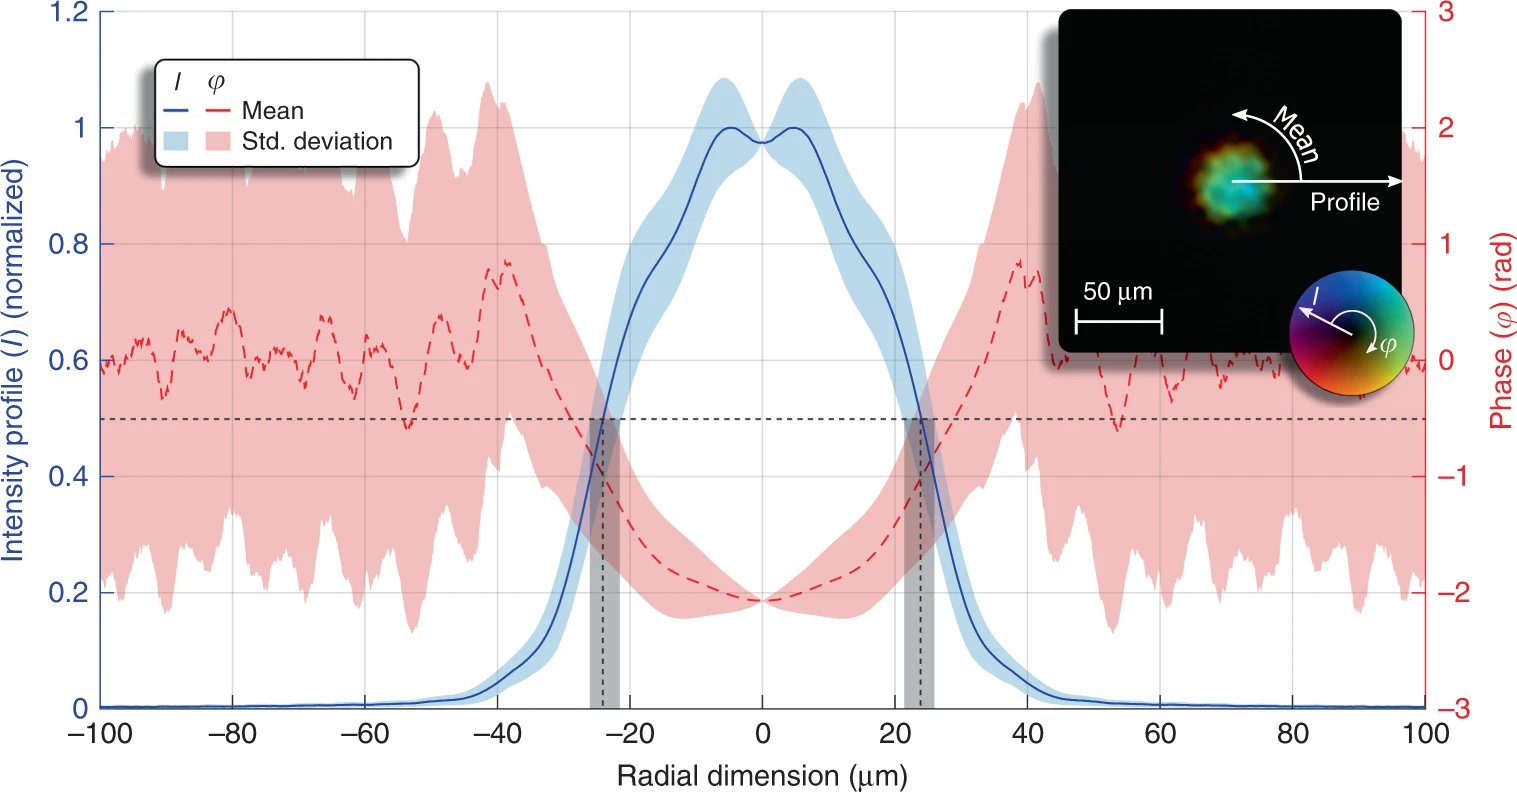
\includegraphics[width=0.8\textwidth]{Figuras/ch2_curvas_lab.png}
  \caption{Perfiles de intensidad (en rojo) y fase (en azul)\autocite{Tuitje2020} obtenidos experimentalmente en el \acrshort{loa}}
  \label{fig:4.1}
\end{figure}

Consecuentemente, para reproducir la pérdida de intensidad en dirección axial, es necesario emplear un ancho del canal con \ce{Kr^{8+}} decreciente en esta misma dirección. A medida que el láser de bombeo \acrshort{nir} viaja a través del canal de plasma, disminuye la intensidad durante su propagación por el medio activo, perdiendo capacidad para generar el ión amplificador \ce{Kr^{8+}} (responsable del efecto láser) y formándose iones inferiores, como \ce{Kr^{7+}}, \ce{Kr^{6+}}, etc. A medida que la semilla alcanza mayores longitudes del canal, la presencia del ión termina reduciéndose a franjas más estrechas ---como muestra la Figura \ref{fig:4.2}---, disminuyendo la amplificación \acrshort{sxrl} obtenida en dirección radial y axial.

Analizando estos elementos, para modelar este ancho variable del canal se propone utilizar una curva logística o sigmoide descrita por la expresión 
\begin{equation}\label{eq:4.0}
  r_{L}(z) = r_{i,min} + \frac{r_{i,max}-r_{i,min}}{1+\eu^{k_{i}(z-z_{0i})}},
\end{equation}
dependiente principalmente de cuatro parámetros: $r_{i,max}$ (valor máximo de la curva), $r_{i,min}$ (valor mínimo de la curva), $k_{i}$ (tasa de decrecimiento o pendiente de la curva) y $z_{0i}$ (coordenada $z$ donde la curva toma su valor medio).

\begin{figure}[htbp]
  \centering
  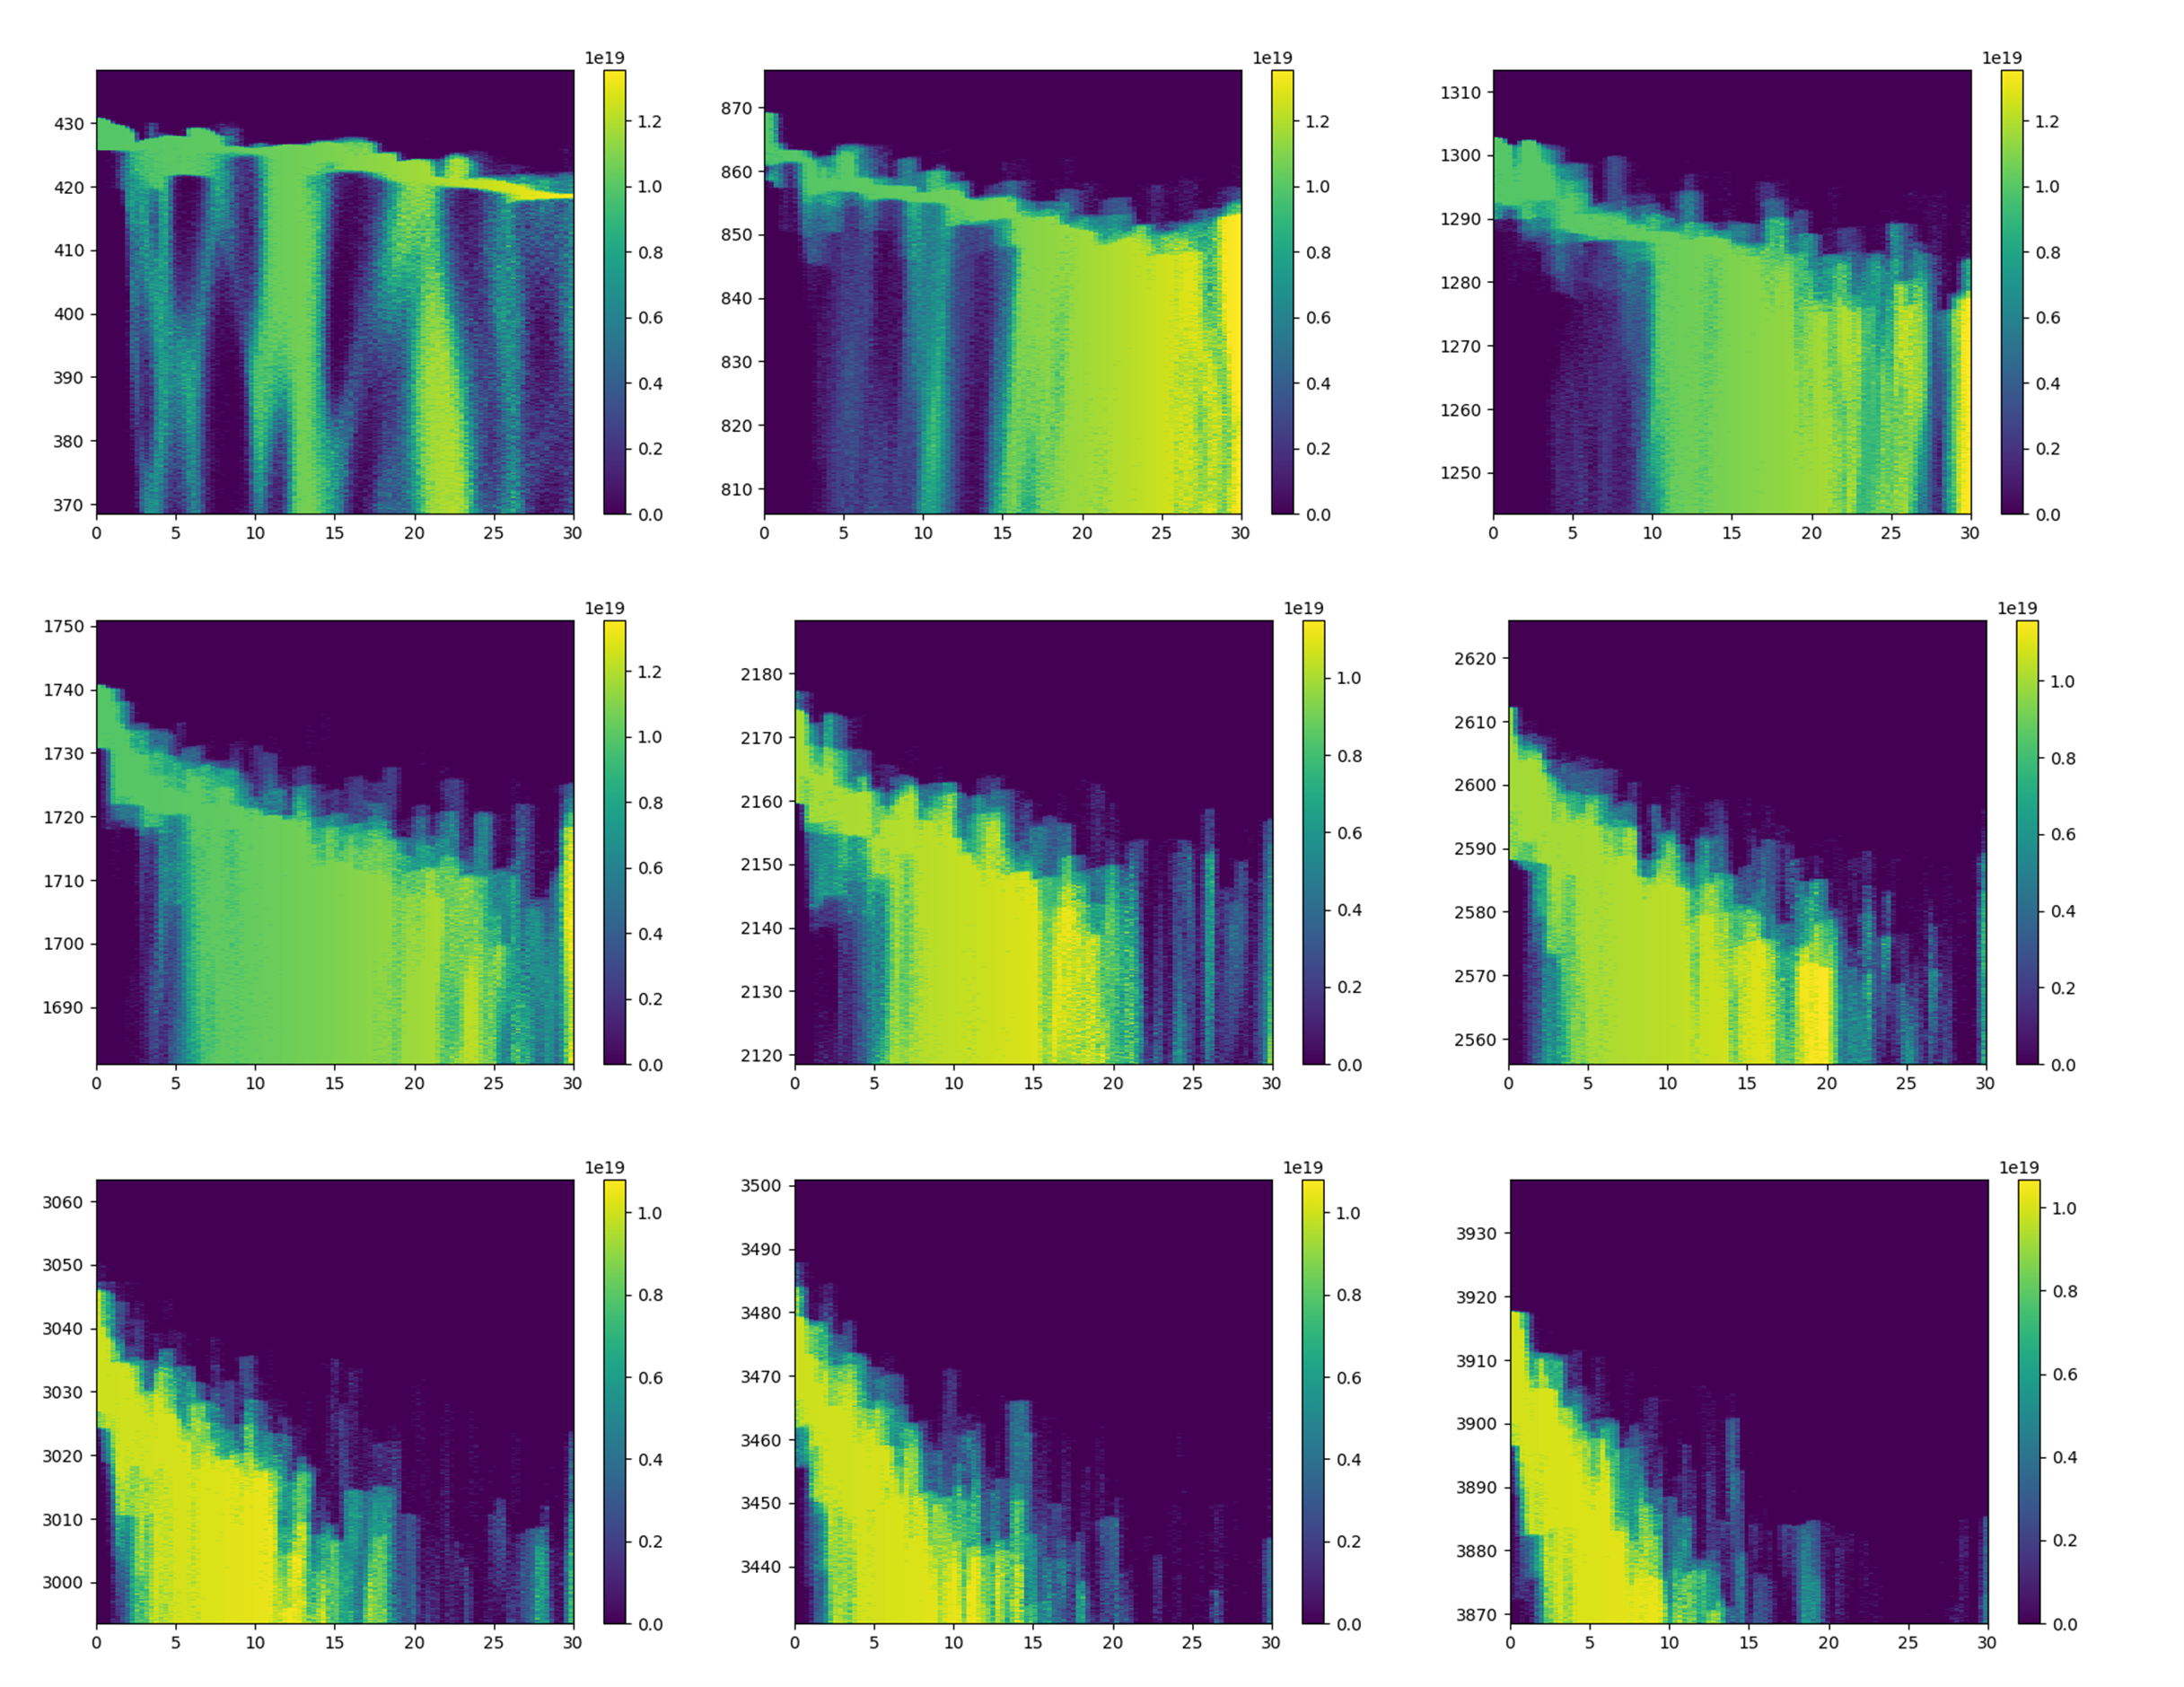
\includegraphics[width=0.8\textwidth]{Figuras/ch4_ionkr8.png}
  \caption{Densidad de \ce{Kr^{8+}} en \unit{cm^{-3}} para diferentes secciones transversales del canal de plasma. El eje horizontal representa la coordenada radial $r$ (\unit{µm}) y el eje vertical la coordenada axial $z$ (\unit{µm})}
  \label{fig:4.2}
\end{figure}

Estos parámetros permiten dar la forma deseada a la frontera del canal con \ce{Kr^{8+}}, controlando la velocidad de la transición entre el valor máximo y mínimo en dirección radial mediante $k_{i}$, además de la posición de la columna de plasma donde comienza el descenso. (recuerda comentar los vaores ue toman las r y qué pasa cuando son 0 o no, hemos ido alternando para ver amplif final e incial)

%\subsection{Variando el parámetro $r_{i,min}$}
%
%\subsection{Variando el parámetro $k_{i}$}
%
%\subsection{Variando el parámetro $z_{0i}$} 
%
%\subsection{Variando el parámetro \texttt{zshift}}

%\section{Con dos sigmoides}\label{sec:4.2}
%
%\subsection{Variando el parámetro $r_{ig,max}$}
%
%\subsection{Variando el parámetro $k_{ig}$}
%
%\subsection{Variando el parámetro $z_{0ig}$} 
%
%\section{Con funciones exponenciales}\label{4.3}
%
%\subsection{Variando el parámetro $r_{u}$}
%
%\subsection{Variando el parámetro \texorpdfstring{$\sigma_{u}$}{sigma-u}}
%
%\subsection{Introduciendo \acrshort{oam}}
%
%\subsection{Eliminando \acrshort{ase}}

